\subsection{AIMed}
AIMed dataset was a result of research in \cite{bunescu2005comparative}.  The authors are 
concerned with automated information extraction from medical texts, especially information about 
human genes/proteins. They chose to think of genes and proteins as interchangeable ideas 
because there is a direct correspondence between them. To obtain the dataset, the authors manually 
tagged about one thousand Medline abstracts \footnote{\url{https://www.nlm.nih.gov/bsd/pmresources.html}}.
They mention following sources of abstracts for human protein interactions:
\begin{enumerate}
  \item 200 abstracts that are known to contain protein interaction from the Database of Interacting Proteins
  \item 30 abstracts for negative examples, where more than one protein mentioned, but there is no interaction between them
\end{enumerate}
In such a way, the AIMed dataset consists of abstracts with marked proteins and protein 
interactions as  pairs. For example

  \begin{verbatim}
    In contrast , in the absence of <prot>  p21ras </prot>  
    , coexpression of <prot>  JAK2 </prot>  and <prot>  
    Raf - 1 </prot>  resulted in an overall decrease in 
    the <prot>  Raf - 1 </prot>  kinase activity .
  \end{verbatim}

has several marked proteins, but no relations. And this

\begin{verbatim}
    Under these conditions , a ternary complex of 
    <p1  pair=6 >  <prot>  p21ras </prot>  </p1>  , 
    <p2  pair=6 >  <prot>  JAK2 </prot>  </p2>  , 
    and  <prot>  Raf - 1 </prot>  was observed .
  \end{verbatim}
  
has three proteins and one interaction pair in it. Since the experiments require sentences with 
only two marked entities the dataset was preprocessed before usage. Each marked entity in the 
sentence was considered as the first entity with each other entity as the second one. Each 
pair was considered only once in the order they are mentioned. An example was marked positive if
proteins were in the same ''pair'' number as ''p1'' and ''p2'' nodes and negative otherwise. In 
the case of presence of ''p1'' or ''p2'' tags, only proteins in these tags were considered, as the 
number of negative samples is significantly larger anyway.  So 
from the first aforementioned sentence six negative examples would be obtained, with entity 
pairs ''p21ras'' - ''JAK2'', ''p21ras'' - ''Raf - 1'' (first occurrence), ''p21ras'' - ''Raf - 1'' (second occurrence), ''JAK2'' - ''Raf - 1'' (first occurrence), ''JAK2'' - ''Raf - 1'' (second occurrence), 
''Raf - 1'' (first occurrence) - ''Raf - 1'' (second occurrence). In the case of the second sentence,
one positive example would be generated with entity pair ''p21ras'' - ''JAK2''.

The dataset is highly unbalanced, having much more negative examples, than positive ones. 
But as all the evaluation tests in other papers are done without balancing, so were held the 
experiments in here.

\subsection{DDI}
The second important relation in medical domain is a drug interaction. The drug interaction is observed 
when one drug influences the level of activity of the other drug \cite{segura20111st}. Knowledge 
about drug 
reactions is critical for patient safety and healthcare costs. There are drug databases, for example, 
DrugBank database \footnote{\url{https://www.drugbank.ca/}}, but data in them is not always up 
to date. 
New information is published regularly in reports and articles. The authors of \cite{segura20111st} are concerned with the application of automatic Natural Language Processing tools for 
extracting knowledge about drug interactions from textual data. Therefore gold standard 
dataset for training machine learning models was created. This dataset 
consists of manually annotated with interactions DrugBank database texts, where drugs were marked by MetaMap 
tool \footnote{\url{https://metamap.nlm.nih.gov/}}. The example of an annotated sentence is:

\begin{verbatim}
<sentence id="DrugDDI.d27.s0" origId="s0" text="The concomitant 
  intake of alcohol and Acamprosate does not affect the 
  pharmacokinetics of either alcohol or acamprosate.">
<entity id="DrugDDI.d27.s0.e0" origId="s0.p1" charOffset="26-33"
 type="drug" text="alcohol"/>
...
<pair id="DrugDDI.d27.s0.p0" e1="DrugDDI.d27.s0.e0" 
e2="DrugDDI.d27.s0.e1" interaction="false"/>
...
</sentence>
\end{verbatim} 

So for each sentence drugs are marked and then all possible pairs with indication of interaction 
between entities - either ''true'' or ''false''. For the test dataset, interaction is set to ''?'' and in separate 
file with gold annotations the labels are written down.

In order to use the dataset each sentence was repeated as many times as it has pairs and for 
each case only one pair of entities was marked. Labels were given according to the 
corresponding interaction label. Again, as with AIMed, the dataset is very unbalanced, having 
more negative examples than positive. But as evaluation papers use exact unbalanced test set 
balancing was not performed.

\subsection{Rosario-Hearst dataset}
This medical dataset was developed for the research in \cite{rosario2004classifying}. Initially, 
the dataset was obtained from MEDLINE abstracts and manually labeled by an expert for seven 
possible relations between DISEASE and TREATMENT. Some of the sentences among the 
examples were also labeled as ''only disease'' or ''only treatment'' and some identified relations, 
such as ''no cure'' had too few examples. Thus the dataset was adapted for making experiments 
with Ranking CNN. First, all not binary relations were filtered out. Then among them only large 
enough were left, they are ''treatment for'' and ''prevents from''. All the other binary relations were 
united for the class ''Other''. Finally, the dataset includes 810 sentences labeled as ''treatment for'', 
63 sentences labeled as ''prevents from'' and 69 for ''Other''. Dataset also contained ''not relevant'' 
examples, i.e. sentences that simply do not contain any entities or relations at all. These examples were outnumbering any of classes, but they could not be used for the experiments with the Ranking Convolutional Neural Network.

This dataset was initially represented as a set of sentences with two (or less) marked entities for each sentence, so the transformation for the experiments was straightforward.

\subsection{Results}
\label{subs:med-superv-res}
 Validation tests were held on AIMed dataset at the same setup as for general domain. But also 
one more choice was tested - usage of general domain embeddings and embeddings trained on 
PubMed abstracts dump from December 2016. The resulting F1 scores could be seen in the 
Table \ref{tab:val-aimed}.

\begin{table}
        \centering
        \begin{tabular}{|c|c|c|c|c|c|c|}
          \hline
            & \multicolumn{6}{|c|}{General domain embeddings} \\\hline
            & \multicolumn{3}{|c|}{Word embedding size 300} & \multicolumn{3}{|c|}{Word embedding size 400} \\\hline
            Dist. emb. & GloVe & Word2Vec & Swivel & GloVe & Word2Vec & Swivel  \\\hline
            \multicolumn{1}{|c|}{30} & 92.295 & 90.04 & 92.12 & 91.86 & 86.72 & 92.76 \\\hline
            \multicolumn{1}{|c|}{40} & 92.49 & 89.74 & 92.05 & 92.09 & 85.49 & 93.00 \\\hline
            \multicolumn{1}{|c|}{50} & 92.36 & 89.19 & 91.87 & 92.09 & 85.13 & 91.27 \\\hline
            \multicolumn{1}{|c|}{70} & 92.62 & 87.65 & 92.07 & 91.797 & 87.099 & 91.32 \\\hline
        \end{tabular}
        
        \begin{tabular}{|c|c|c|c|c|c|c|}
          \hline
            & \multicolumn{6}{|c|}{Medical domain embeddings} \\\hline
            & \multicolumn{3}{|c|}{Word embedding size 300} & \multicolumn{3}{|c|}{Word embedding size 400} \\\hline
            Dist. emb. & GloVe & Word2Vec & Swivel & GloVe & Word2Vec & Swivel  \\\hline
            \multicolumn{1}{|c|}{30} & 91.97 & 91.71 & 92.43 & 91.65 & 91.56 & \textit{93.25} \\\hline
            \multicolumn{1}{|c|}{40} & 92.44 & \textit{92.13} & \textit{92.72} & \textbf{93.38} & 91.23 & 92.46 \\\hline
            \multicolumn{1}{|c|}{50} & 92.19 & 91.397 & 92.51 & 91.85 & 91.92 & 92.55 \\\hline
            \multicolumn{1}{|c|}{70} & \textit{92.84} & 90.95 & 92.47 & 92.19 & \textit{92.197} & 91.7 \\\hline
        \end{tabular}
        \caption[Cross-validation for the medical domain]{Results of the cross-validation experiments on AIMed dataset obtained by simple calculation of F1-score for binary case. Every score is an averaged score of four 
experiments. First table contains results for general domain embeddings, second for medical 
domain. With \textit{italics} marked scores maximal in the column and \textbf{bold} is for the 
maximal result overall.}
        \label{tab:val-aimed}
    \end{table}

All the training accuracies reached 100 percent, sometimes after 4-5 epochs, except for experiments with Word2Vec of length 400 trained on general domain. In those experiments accuracy was reaching 94-96 percents.
From the results of the evaluation, it can be seen that embeddings trained on medical domain always 
give better result. The highest results are also always obtained with GloVe embeddings, while changing 
the dimensionality of word embeddings does not critically change the score. Change in the size 
of distance embeddings causes worse results when getting higher than 50. As the best model 
was chosen the one with GloVe medical embeddings of size 400 and with distance embeddings 
of 40.

As in the original paper \cite{bunescu2005comparative} results were obtained by 10-fold 
cross-validation and models in several other papers were as well 
(\cite{bunescu2005subsequence}, \cite{airola2008all}) evaluated in this way, the test for AIMed 
dataset was also performed with original 10-fold split. The DDI dataset also contains direct split on 
training and testing articles, so all the sentences formed from the testing articles were used as a 
testing set. The Rosario-Hearst dataset was simply split to 75\% of training data and 25\% of testing 
data and evaluation was held on the testing data. The results of testing 
the network are in the Tables \ref{tab:test-aimed}, \ref{tab:test-ddi}, \ref{tab:test-ros-hearst}.

\begin{table}[h]
  \begin{center}
 \begin{tabular}{ | c | c | c | c | }
    \hline
    Classifier & P & R & F1 \\ \hline
    Original paper best result \cite{bunescu2005comparative} \footnote{As in both \cite{bunescu2005comparative} and \cite{bunescu2005subsequence} authors gave PR-curve for result evaluation here was used the point corresponding to P=55.69 as obtained by the Ranking CNN.} & 55.69 & 36 & 43.73 \\\hline
    Subsequent kernels \cite{bunescu2005subsequence} & 55.69 & 54 & 54.83 \\\hline
    Graph kernel \cite{airola2008all} & 52.9 & 61.8 & 56.4  \\ \hline
    Supervised Ranking CNN (balanced train) \footnote{Training was performed on the dataset where number of negative and positive examples was balanced by cutting off negative examples.} & 34.27 & \textbf{90.56} & 49.29 \\ \hline
    Supervised Ranking CNN  & 55.69 & 63.85 & \textbf{58.38}  \\ \hline
    \end{tabular}
    \caption[Medical domain, AIMed evaluation results]{Results of evaluation of the network with AIMed.}
\label{tab:test-aimed}
\end{center}
\end{table}

\begin{table}
  \centering
     \begin{tabular}{ | c | c | c | c | }
    \hline
    Team \footnote{Results of competition from the original paper \cite{segura20111st}} & P & R & F1 \\ \hline
    WBI &  60.54 & 71.92 & 65.74 \\ \hline
    FBK-HLT &  58.39 & 70.07 & 63.70 \\ \hline
    Uturku &  58.04 & 68.87 & 62.99 \\ \hline
    LIMSI-CNRS &  55.18 & 64.90 & 59.65 \\ \hline
    laberinto-uhu &  50.00 & 44.37 & 47.02 \\ \hline
    Supervised Ranking CNN (balanced train) & 22.38 & \textbf{100.00} & 36.58 \\ \hline
    Supervised Ranking CNN & \textbf{91.75} & 98.68 & \textbf{95.09} \\ \hline
    \end{tabular}
  \caption[Medical domain, DDI evaluation results]{Results of evaluation of the network with DDI.}
\label{tab:test-ddi}
\end{table}

\begin{table}
  \begin{center}
      \begin{tabular}{ | c | c | c | c | }
    \hline
    Classifier & P & R & F1 \\ \hline
    Supervised Ranking CNN & 90.05 & 82.14 & 85.58 \\ \hline
    \end{tabular}
\caption[Medical domain, Rosario-Hearst evaluation results]{Results of evaluation of the network with Rosario-Hearst dataset.}
\label{tab:test-ros-hearst}
\end{center}
\end{table}

For the training datasets, all the experiments were getting 100 percent accuracy. 

It is interesting to notice, that training on the balanced dataset while testing still on unbalanced 
leads to higher Recall, but lower Precision. It directly reflects the idea, that distribution of both 
training and testing sets should be the same, otherwise supervised learner will not be able to 
be precise. So having a balanced training set, model suggests that much more examples are 
positive in the testing set than it really is - from what follows high Recall. But this time it is not the 
case and that is why Precision is low.

Also, it should be noticed, that in the AIMed and DDI datasets one and the same sentence will be an 
example for both negative and positive labels. And of course, it is hard for the network to extract 
syntactic construction that will be a sign of positive relation. 

So it can be concluded, that the model gives state-of-the-art results for various medical 
datasets with different classes of relations. Compared to the evaluation from several other authors Ranking
CNN gives always a better result. 


\subsection{Interpretation}
\paragraph{Representative trigrams extraction} 
In order to see the effect of balancing datasets, several sets of representative trigrams were 
extracted. 

The first one is for the network trained on the balanced AIMed dataset, second one is for the unbalanced 
dataset and the third one was made as a separate experiment, where dataset was initially 
balanced and then split on 75\% for training and 25\% for testing. The result shown by this 
training was P=51.91, R=92.08, F1=66.39.

\textbf{Balanced dataset} \textit{interaction with p25shc, binding, complex, interaction}

\textbf{Unbalanced dataset} \textit{interaction of the, interaction with p25shc, binding, binding region of}

\textbf{Initially balanced dataset} \textit{tr6 specifically binds, interacts poorly with, interacts with the, interaction}

From the human point of view, all the sets capture a lot of meaningful expressions of interaction.

The same three sets were obtained for DDI dataset. The scores for the network trained on 
the initially balanced dataset are P=59.68, R=98.84, F1=74.42, so it performs better than on 
AIMed dataset. But of course, it should be noticed that in general results for DDI dataset are also 
higher.

\textbf{Balanced dataset} \textit{of aprepitant with, hormonal contraceptives may, of erythromycin and, taking tarceva with, of erythromycin with, probenecid is, amphetamines may, azithromycin had, the benzodiazepines may}

\textbf{Unbalanced dataset} \textit{etonogestrel may interact, monoamine oxidase inhibitors, barbiturates, of erythromycin with, of amphetamines, nsaids can reduce, carbamazepine, may inhibit, nsaids may diminish}

\textbf{Initially balanced dataset} \textit{caution, agents, drugs, inhibitors, amphetamines, levels}

For DDI dataset most meaningful are trigrams extracted for the unbalanced training set. It can be explained by considering the fact, that the unbalance in amounts of negative and positive examples for this dataset are higher (almost 15 times more negative examples), than for the AIMed (around 3 times more negative examples). So when balancing is performed, network learns more drug names that can affect each other, rather than syntactic constructions denoting interactions.

\paragraph{Semantic values} 
For checking how the network ''sees'' the sentence in terms of values for the final decision 
two examples from AIMed test dataset were taken. The first one was classified correctly and the 
second one was mistakenly classified as ''Interaction''. The sentences are:

\begin{itemize}
  \item "Our data suggest that TR6 inhibits the interactions of $<e1>$LIGHT$</e1>$ with $<e2>$HVEM$</e2>$ / TR2 and LTbetaR, thereby suppressing LIGHT - mediated HT29 cell death."
  \item "We have previously identified $<e1>$IL - 11$</e1>$ specific binding protein which is distinct from that of $<e2>$IL - 6$</e2>$ in a number of cell lines."
\end{itemize}

Corresponding plots for these examples can be seen in the Figure \ref{fig:aimed-semantic-val}. The 
first sentence classified correctly as denoting ''Interaction'' and it can be seen that there are  
spikes over \textit{inhibits} and \textit{interactions of} and \textit{with}. As the value calculated for the trigram, it would be visualised over the central word of it. Thus, spike in the centre over \textit{/} is a spike over a protein name \textit{hvem/tr2}. That denotes that network is learning entities names as well. The second example is classified wrongly as describing interaction. 
The plot has numerous spikes over names of proteins and over \textit{specific binding protein} that leads to the high score for the 
''Interaction'' class, while these exact proteins do not interact.

Additionally, it is seen, that with longer sentences semantic values become much smaller (compare to 
analogous evaluation for SemEval2010 dataset in general domain) because they are distributed 
among all the words and thus it is harder to extract needed parts. Due to this spikes over the beginning and the end of 
an example become more prominent. They appear because sentences are padded with zero values for convolution and the 
activation function is tanh. Thus, zeroes can get higher values than some other words in the sentence with negative 
values.

\begin{figure}[H]
  \tiny
\centering
\subfigure[LIGHT - HVEM]{
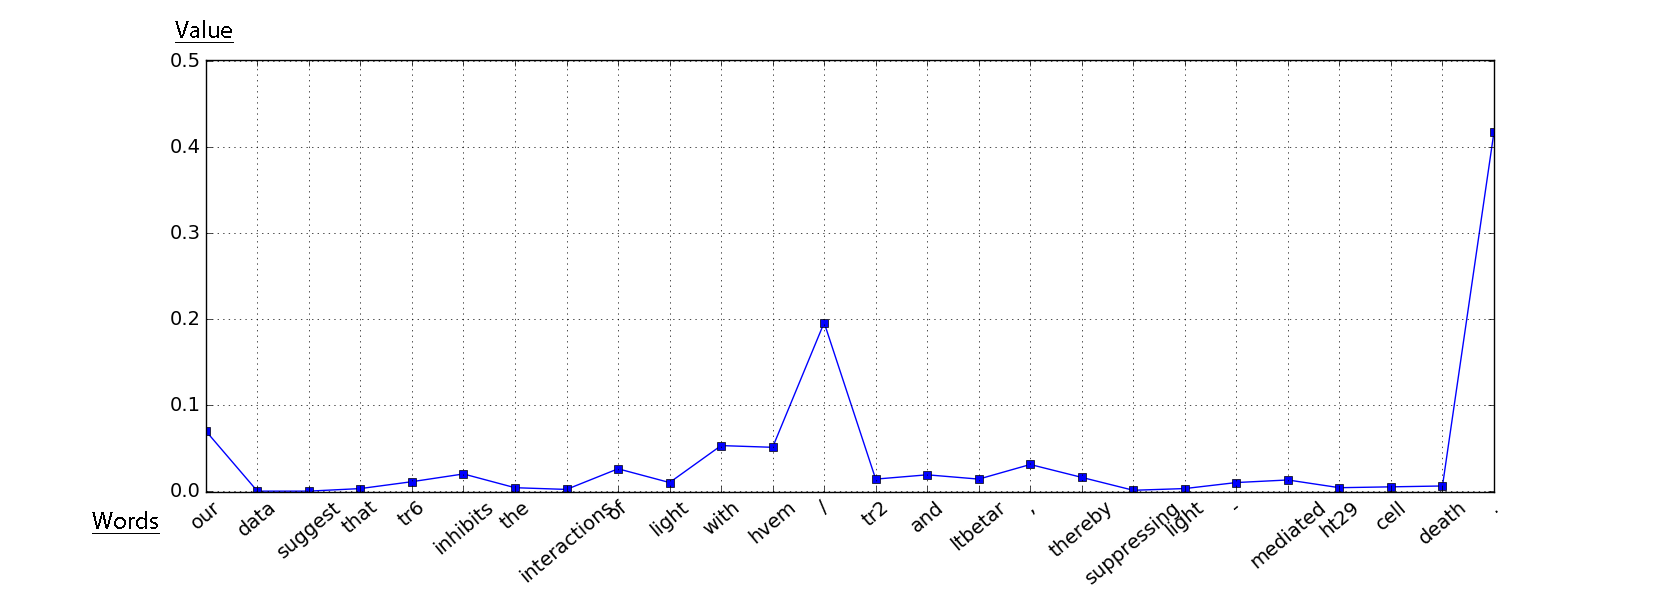
\includegraphics[width=\textwidth]{chapter4_experiments/images/aimed-sem-val1.png}
}
\subfigure[IL-11  - IL-6]{
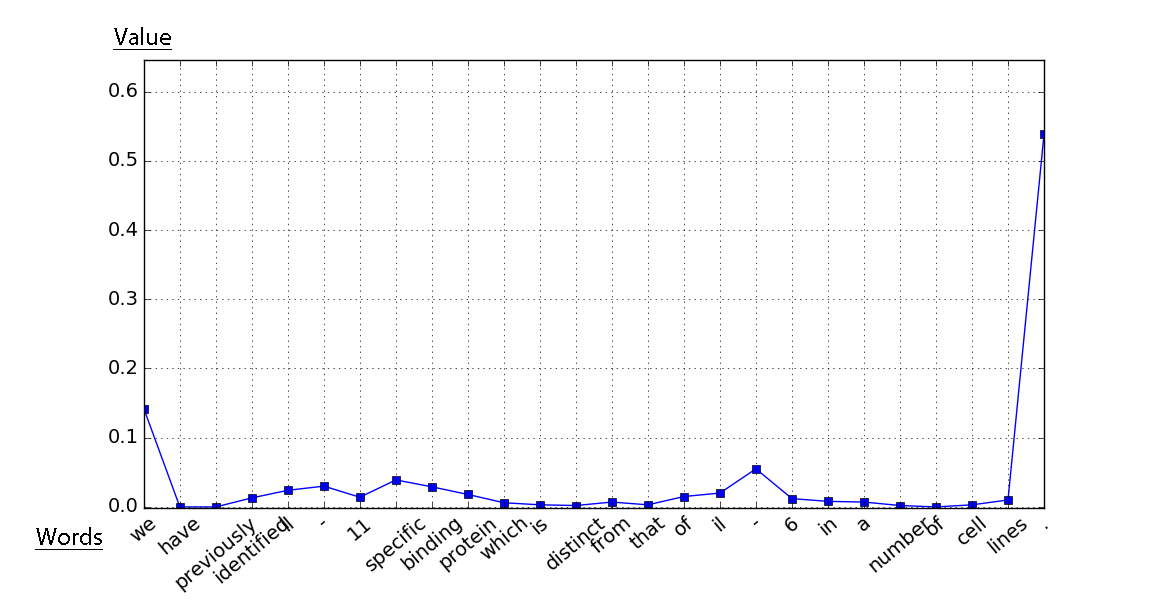
\includegraphics[width=0.75\textwidth]{chapter4_experiments/images/aimed-sem-val2.png}
}
\caption[Semantic values, medical domain supervised experiments]{ Semantic values for classification of the words in sentences. }
\label{fig:aimed-semantic-val}
\end{figure}

\paragraph{Scores distribution}
Corresponding scores distribution plots for the same two examples can be seen in the Figure 
\ref{fig:aimed-scores-distr}. The first example was recognised correctly and the network is quite 
sure in its answer. The second one was recognised 
incorrectly with a rather high certainty as well. This again can be explained by the spikes on the protein names 
that are seen on the semantic evaluation plot for the second example.

\begin{figure}[H]
\centering
\subfigure[Interaction]{
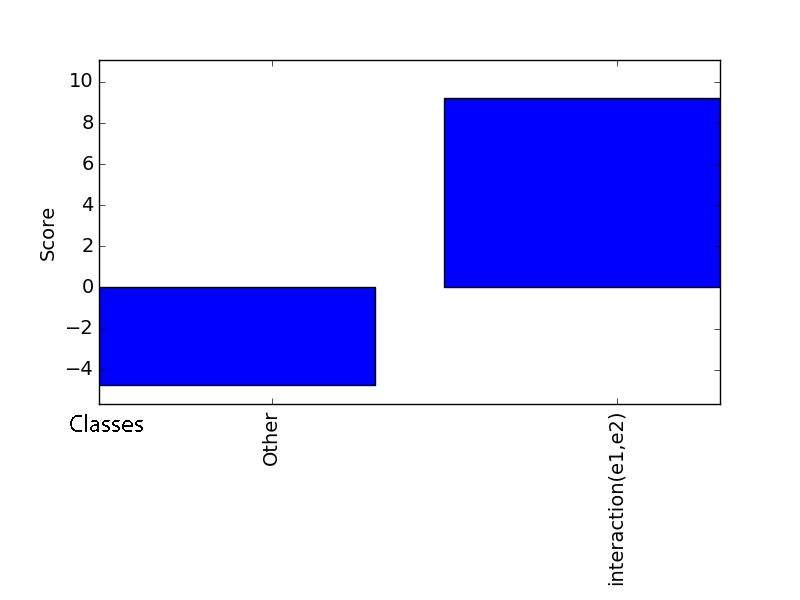
\includegraphics[width=.47\textwidth]{chapter4_experiments/images/aimed-scores1.png}
}
\subfigure[Other]{
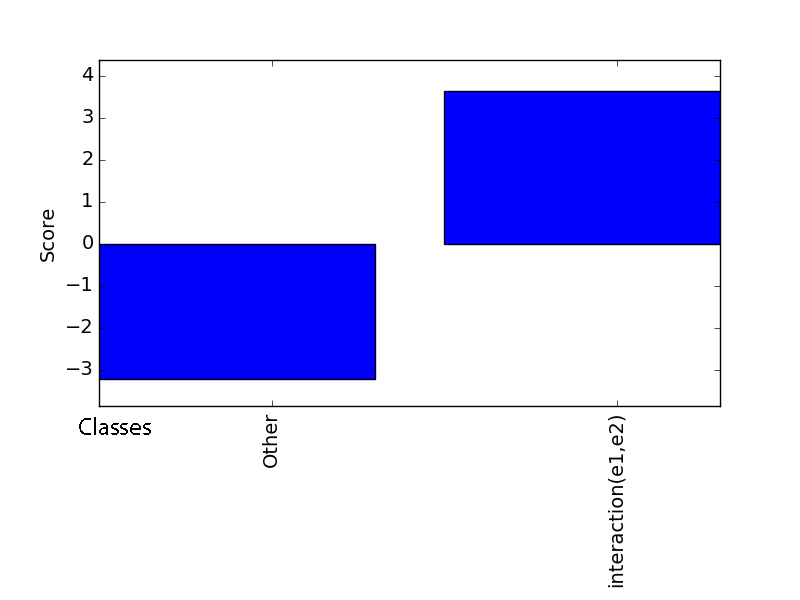
\includegraphics[width=.47\textwidth]{chapter4_experiments/images/aimed-scores2.png}
}
\caption[Scores distributions, medical domain supervised experiments]{Distribution of scores values.}
\label{fig:aimed-scores-distr}
\end{figure}
